% - Why is asset allocation important? Short description of the asset allocation optimisation problem.
% - Short history of Markowitz's Modern Portfolio Theory.

Assume an investor with a total wealth of $\$x \in \mathbb{R}_{\geq 0}$, i.e. a total wealth of $x$ U.S. dollars. Let $A := \{a_1, \dots, a_N \}$ be the set of assets, which the investor can trade, such that $a_i$ is the real-valued random variable representing the return of asset $i = \{ 1, \dots, N \}$. By asset, we understand anything with a price that can be bought and sold so as to profit from price differences across time, i.e. returns. However, here we will focus on the most widely used investment assets: for example cash, real-estate objects, bonds, stocks, commodities and funds.

\begin{definition}
    A \textbf{portfolio $P_A$ composed of the assets $A$} is defined as
    \begin{align*}
        P_A := \begin{bmatrix} w_1 \\ \vdots \\ w_N \end{bmatrix} \in \mathbb{R}^N, \quad \text{such that} \quad \sum_{i=1}^N w_i = 1
    \end{align*}
    where each weight $w_i$ represents the relative allocation of the investor's total wealth to asset $i = \{ 1, \dots, N \}$. The real-valued random variable of the portfolio return $X$ is given by
    \begin{align*}
        X = \sum_{i=1}^N w_i a_i
    \end{align*}
\end{definition}

One of the most important questions that an investor faces is how much of their total wealth $\$x$ they should allocate to each of the assets in $A$, i.e. which portfolio $P_A \in \mathbb{R}^N$ they prefer to hold. This question has infinite discretionary and many systematic answers. Harry M. Markowitz was the first to develop and present a systematic approach to this asset allocation problem by defining it as an optimisation problem with 2 variations in 1952 \cite{markowitzorg}:
\begin{enumerate}
    \item Maximise returns while maintaining risk within a given risk tolerance level, or
    \item Minimise risk for a given level of target return.
\end{enumerate}
Moreover, he defined risk as the standard deviation of past returns and returns as the expected value of past return. His work earned him a Nobel Memorial Prize in Economic Sciences in 1990 \cite{markowitznobelprize}. Markowitz's portfolio construction model laid the ground for quantitative asset allocation models. Many asset allocation models today are developed using Markowitz's model and adjusting it to account for modern investors' needs. For example, by using risk measures other than the standard deviation of past returns, or by targeting functions other than expected returns.

The main critique point of Markowitz's portfolio construction model is the lack of stability that leads to a high portfolio turn-over and to concentrated portfolios, especially when correlations rise. Here, we analyse Markowitz's portfolio construction model and the causes of low stability by focusing on the minimum volatility portfolio. Moreover, we present some techniques that try to improve the stability of minimum volatility portfolios: one regarding parameter estimation for Markowitz's model and one alternative allocation method. Moreover, we also compare Markowitz's minimum volatility portfolios to two naive allocation methods: equal weight and inverse variance allocation.

\subsection{Practical Implementation Framework}
    % for example, the time period of the backtest, the rebalancing frequency, the data resolution, transaction costs, etc.
    
    To show the problems of Markowitz's minimum volatility portfolios in real applications, and compare these portfolios to the portfolios computed using the other methods and techniques, each of the techniques described here is implemented for a portfolio of exchange traded products (ETPs) representing 4 assets classes: equities, fixed income, real estate and commodities \footnote{See appendix \ref{Selected_ETPs} for a detailed description of the $N=20$ selected ETPs and the selection process.}. We use the QuantConnect platform \cite{qcwebsite} for the implementation and as the data source. This platform and its API allow us to perform backtests with one-minute resolution data. A backtest is nothing else than a simulation of a portfolio with past data to see how it would have behaved, if we had hold it during that past period considered in the backtest. With one-minute resolution data, we have price data that is sampled once per minute. This allows us to model the changes in portfolio value as well as the entry and closing price of orders accurately considering the fact that the holding period is at least one month.
    
    \subsubsection{Backtest Settings}\label{backtestsettingssec}
        In total, 12 portfolios are computed, corresponding to a backtesting period from January 1, 2020 to December 31, 2020 and monthly rebalancing-interval. The rebalancing occurs on the first trading day of each month at 10:00 AM New York time. An initial account balance of 10 million U.S. dollars is assumed, and margin calls are deactivated in order to better simulate the theoretical portfolios computed.
        
        For the computation of portfolio weights, the daily returns of the past 60 days is used as input. This last setting does not affect the equal weight portfolio construction method, because this naive method does not use any past data as input. The reason why we use 60 days of past data is because we need at least 20 periods of data to fulfil a necessary condition for the invertibility of the sample covariance matrix, and 60 days corresponds to 3 full trading months of data.
        
        \begin{definition}[Sample Covariance, Variance, Standard Deviation and Correlation Matrices of Asset Returns]\label{covmatrixdefition}
           Let $R := [r_{n,t}]_{n = 1, \dots, N; t = 1, \dots, T} \in \mathbb{R}^{N \times T}$ be the matrix that contains $T \in \mathbb{N}$ observations of the $\{ a_1, \dots, a_N \}$ real-valued random variables of asset returns. Moreover, let the matrix of centred returns be defined as
           \begin{align*}
               \tilde{R} := [\tilde{r}_{n,t}] \in \mathbb{R}^{N \times T} \quad \text{where} \quad \tilde{r}_{n,t} = r_{n,t} - \frac{1}{T} \sum_{i=1}^T r_{n,i}
           \end{align*}
           Then, the \textbf{$T$-periods sample covariance matrix of asset returns} $\Sigma := [\sigma_{i,j}] \in \mathbb{R}^{N \times N}$ is defined as
           \begin{align*}
               \Sigma := \frac{1}{T} \left( \Tilde{R}^T \cdot \Tilde{R} \right)
           \end{align*}
           where $s_{i,j}$ represents the $T$-periods sample covariance of the $i$-th and $j$-th assets. Finally, we define the \textbf{variance matrix} $V = [v_{i,j}] \in \mathbb{R}^{N \times N}$, the \textbf{standard deviation matrix} $S = [s_{i,j}] \in \mathbb{R}^{N \times N}$ and the \textbf{correlation matrix} $P = [\rho_{i,j}] \in \mathbb{R}^{N \times N}$, where
           \begin{align*}
               v_{i,j} &:= \begin{cases}
                    \sigma_{i,j}            &\quad \text{for } i=j \\
                    0                       &\quad \text{else}
               \end{cases} \\
               s_{i,j} &:= \begin{cases}
                    \sqrt{\sigma_{i,j}}     &\quad \text{for } i=j \\
                    0                       &\quad \text{else}
               \end{cases} \\
               P &= S^{-1} \Sigma S^{-1}
           \end{align*}
        \end{definition}
        
        \begin{remark}
            Because we don't know the mean return of each asset and use the sample mean to compute the sample covariance matrix, we need to use Bessel's correction to get an unbiased estimator of the sample covariance matrix. That is an estimator that is equal to its expected value. Let $T > 1$ and $\Sigma, V, S$ be the sample covariance, variance and standard deviation matrices defined above respectively, their unbiased estimator is given as
            \begin{align*}
                \Sigma_{unbiased} &:= \frac{T}{T-1} \Sigma \\
                V_{unbiased} &:= \frac{T}{T-1} V \\
                S_{unbiased} &:= \frac{T}{T-1} S
            \end{align*}
            From now on, when we refer to the sample covariance, variance and standard deviation matrices, we refer to them after Bessel's correction.
        \end{remark}
        
        \begin{theorem}
            Let $R, \tilde{R}, \Sigma$ be defined as in definition \ref{covmatrixdefition}. If $\Sigma \in GL_N(\mathbb{R})$, then $rank(R) = N$ holds.
        \end{theorem}
        
        \begin{proof}
            If $\Sigma \in GL_N(\mathbb{R})$, then
            \begin{align*}
                N = rank(\Sigma) \leq rank \left( \frac{1}{T} \left( \Tilde{R}^T \cdot \Tilde{R} \right) \right) \leq rank(\Tilde{R}) \leq rank(R) \leq \min \{ N, T \}
            \end{align*}
            Hence, $rank(R) = N$ and $N \leq T$ must hold. The same also applies to the unbiased sample covariance matrix for $T > 1$.
        \end{proof}
        
        In our practical implementation framework, we have selected $N = 20$ assets, therefore $T \geq 20$ must hold. This does however not guarantee that the covariance matrix has full rank and hence is invertible, because the condition $N \leq T$ is not a sufficient condition for that.
		
		There is not a single true underlying covariance matrix, but rather one that changes over time according to human behaviour and psychology, else every investor could compute optimal portfolios that would remain optimal over time. Therefore, it is worth to mention the trade-off between higher values of $T$, which lead to a more stable, with higher probability non-singular sample covariance matrix over time but at the same time make the portfolio optimisation less sensitive to changes in market trends and regimes, and lower values of $T$, which make the covariance matrix estimation process more sensitive to changes in market trends and regimes but make the portfolio optimisation process less stable. The asset manager should always take this into account, in order to reduce noise in the estimation while still using input parameters that allow to react to changes in the market. In the case of our practical implementation framework, we could, of course, have chosen a different value of $T$, and there is no mathematical reason to prefer $T=60$ to $T=59$ or $T=100$, for example. However, optimising the covariance matrix estimation process with respect to the number of observations used for its computation is not part of this work, and a 3-month past-data-window seems acceptable for the estimation of portfolios with a holding period of one month (optimal portfolios are computed and rebalanced each month).
    
    \subsubsection{Portfolio Analyses}
        
        % Tools to analyse PFs: HHI for concentration, risk-adjusted returns, stability: turn-over volume, what else?
        
        The portfolios generated by each optimisation method in backtesting will be analysed with respect to risk-adjusted return, concentration and stability. The Sharpe ratio is the chosen measure to quantify risk-returns. To assess concentration, we will use a normalised version of the Herfindahl-Hirsch-Index (HHI). The normalisation step is necessary, because we will allow for short positions in our portfolios, and the HHI is only defined for positive portfolio weights. We will measure stability via the turnover of the portfolio.
        
        \begin{definition}[Sharpe Ratio \cite{franzen}] % Page 216
            Let $\mu_P \in \mathbb{R}$ be the return of the portfolio $P$ over a given period of time and $\sigma_P \in \mathbb{R}_{\geq 0}$ its standard deviation over that same period of time. Moreover, let $R_f \in \mathbb{R}$ be the risk-free rate of that given period. Then the \textbf{Sharpe Ratio of portfolio $P$ over the given period} $SR_P \in \mathbb{R}$ is given by
            \begin{align*}
                SR_P := \frac{\mu_P - R_f}{\sigma_P}
            \end{align*}
        \end{definition}
        
        \begin{remark}
            We do not compute the Sharpe ratio of the backtest separately, and rely upon QuantConnect's internal overall portfolio statistics for its computation, i.e. all Sharpe ratios presented here are the Sharpe ratios that appear in QuantConnect's backtesting results. QuantConnect computes the Sharpe ratio using the same definition as above, but using the annualised return of the portfolio in the backtest \cite{qcsharperatiocode}.
        \end{remark}
        
        % https://quant.stackexchange.com/questions/65525/herfindahl-hirsch-index-for-fx-portfolios?noredirect=1#comment92677_65525
        %To assess concentration, we choose Yager's entropy, because, in contrast to the Herfindahl-Hirsch-Index, Yager's entropy allows asset weights to be negative. 
        
        %\begin{definition}[Yager's Entropy \cite{yagerentropy}]
        %    Consider a portfolio with $n$ assets. Let $w_1, \dots, w_n \in \mathbb{R}$ be the weights associated to each of the $n$ assets in the portfolio. Then Yager's entropy $Q(w_1, \dots, w_n)$ is defined as
        %    \begin{align*}
        %        Q(w_1, \dots, w_n) := - \left( \sum_{i=1}^n \left| w_i - \frac{1}{n} \right|^z \right)^{\frac{1}{z}}
        %    \end{align*}
        %    where $z \in \mathbb{N}_{\geq 1}$ is a constant. \todo{change source to \url{https://www.sciencedirect.com/science/article/abs/pii/002002559400030F}}
        %\end{definition}
        
        %\begin{remark}
        %    \todo{add remark, that min entropy if equal weighted portfolio}
        %\end{remark}
        
        \begin{definition}[Herfindahl-Hirsch-Index \cite{chammas}] % Page 71 (85 of the PDF)
            Let $P$ be a portfolio containing $N$ assets with weights $w_i \in \mathbb{R}_{\geq 0}$ for all $i=1, \dots, N$, such that $\sum_{i=1}^N w_i = 1$. We define the \textbf{Herfindahl-Hirsch-Index (HHI)} as
            \begin{align*}
                HHI_P := \sum_{i=1}^N w_i^2
            \end{align*}
            For the general case of a portfolio $P$ with weights $w_i \in \mathbb{R}$ for all $i = 1, \dots, N$, we define the \textbf{normalised Herfindahl-Hirsch-Index (nHHI)} as
            \begin{align*}
                nHHI_P := \sum_{i=1}^N \left( \frac{|w_i|}{\sum_{j=1}^N |w_j|}\right)^2
            \end{align*}
            Obviously, $nHHI_P \leq HHI_P$ for the general case of a portfolio $P$ with weights $w_i \in \mathbb{R}$ for all $i = 1, \dots, N$.
        \end{definition}
        
        \begin{definition}[Turnover \cite{equalweight}]
            Consider a portfolio $P$ with $N$ assets. Let $w_{j,t+1} \in \mathbb{R}$ be the portfolio weight assigned to asset $i$ at time $t$ by the portfolio optimisation method, and let $w_{j,t^+} \in \mathbb{R}$ be the portfolio weight of asset $i$ before rebalancing at time $t+1$ for $i=1, \dots, N$ and $t=0, \dots, T$. The turnover of the portfolio $P$ is defined as
            \begin{align*}
                TO_P := \frac{1}{T} \sum_{t=0}^T \sum_{i=1}^N \left( \left| w_{i, t+1} - w_{i, t^+} \right| \right)
            \end{align*}
            where $T \in \mathbb{N}$ is the number of rebalancing points of the portfolio.
        \end{definition}
        
        This turnover quantity can be interpreted as the average percentage of wealth traded at each rebalancing point.
        
    \subsubsection{Benchmark Portfolio Construction Methods}
        We use 2 naive portfolio allocation models, equal weight and inverse variance allocation, as benchmarks for the other 3 methods (Markowitz minimum volatility portfolio, Markowitz minimum volatility portfolio with covariance matrix shrinking and hierarchical risk parity) to estimate if the the increased complexity of the latter can be justified in form of better risk-adjusted returns, concentration and stability.
        
        \begin{definition}[Equal Weight Portfolio \cite{equalweight}]
            Consider the set of investable assets $A := \{ a_1, \dots, a_N \}$. The \textbf{equal weight allocation portfolio (EWP)} is defined as
            \begin{align*}
                EWP_A := [w_i]_{i=\{1, \dots, N \}} \quad \text{such that} \quad w_i := \frac{1}{N} \quad \text{for all} \quad i = 1, \dots, N
            \end{align*}
        \end{definition}
        
        The equal weight portfolio is the most widely used allocation method when no information about the assets in the portfolio is available to rank them or to compute some measure to define an optimisation problem. It is also the most naive way of allocating capital across the $N$ assets considered. However, this naive method has proven to perform even better than other, even very sophisticated, methods \cite{equalweight}.
        
        \begin{definition}[Inverse Variance Portfolio \cite{equalweight}]\label{definition:inversevarianceportfolio}
           Consider the set of investable assets $A := \{ a_1, \dots, a_N \}$. The \textbf{inverse variance allocation portfolio (IVP)} is defined as
            \begin{align*}
                IVP_A := [w_i]_{i=\{1, \dots, N \}} \quad \text{such that} \quad w_i := \frac{\frac{1}{\mathbb{V}[a_i]}}{\sum_{k=1}^N \frac{1}{\mathbb{V}[a_k]}} \quad \text{for} \quad i=1, \dots, N
            \end{align*}
            where $\mathbb{V}[a_i]$ is the variance of the returns' distribution of the $i$-th asset.
        \end{definition}
        
        The IVP can be understood as the allocation method that weights each asset in the portfolio so that each of them contributes the same amount to the total portfolio risk (assets with higher variance are allocated a smaller portion of the portfolio than assets with lower variance).
        
        Although IVP is more complex than the equal weight allocation  model because the estimation of some parameters is needed, it is still considered a naive method.
        
        The vectors with the optimal portfolios computed using these 2 naive methods can be found in appendices \ref{EW_Portfolios} and \ref{IV_Portfolios}. In figure \ref{fig:ivp_allocation_plot}, a visual representation of the target allocation of all 20 assets in the IVP over the backtesting period is presented. Most of the portfolio's wealth is allocated to ISTB (iShares Core 1-5 Year USD Bond ETF) and IAGG (iShares Core International Aggregate Bond ETF). The allocation to the first drops at the start of the COVID-19 crisis, while the allocation of the second rises. The allocation to IMTB (iShares 5-10 Year USD Bond ETF) rises after the start of the COVID-19 crisis. For the rest of assets the allocation remains relatively stable over the whole backtesting period. Finally, the high allocation to fixed income ETFs is not surprising, because they tend to present lower variance of returns, while the allocation to equity, including real-estate, and commodity ETPs remains low due to the higher variance of returns that they tend to present.
        
        % Data
        \begin{figure}[p]
            \centering
            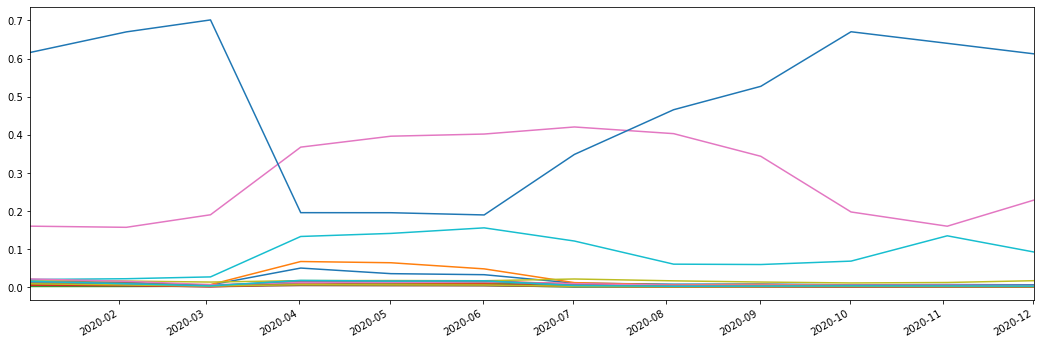
\includegraphics[width=1.15\textwidth]{bilder/IVP_allocation_plot.png}
            \caption{IVP Target Allocation over Time}
            \label{fig:ivp_allocation_plot}
        \end{figure}
        
        A similar plot for the EWP target allocation over time is not necessary, since the target allocation to each asset is equal and remains the same over the whole backtesting period.
        
        Figure \ref{fig:nHHI_EWP_and_IVP} shows the evolution of the nHHI of the 2 naive portfolio allocation models described above. The nHHI of the equal weight portfolios is low and stays the same over time, as expected. In the case of IVP, the nHHI rises with the start of the COVID-19 crisis to latter more than halve, mostly because of a reduction in the allocation to ISTB as explained previously.
        
        % Data
        \begin{figure}[p]
            \centering
            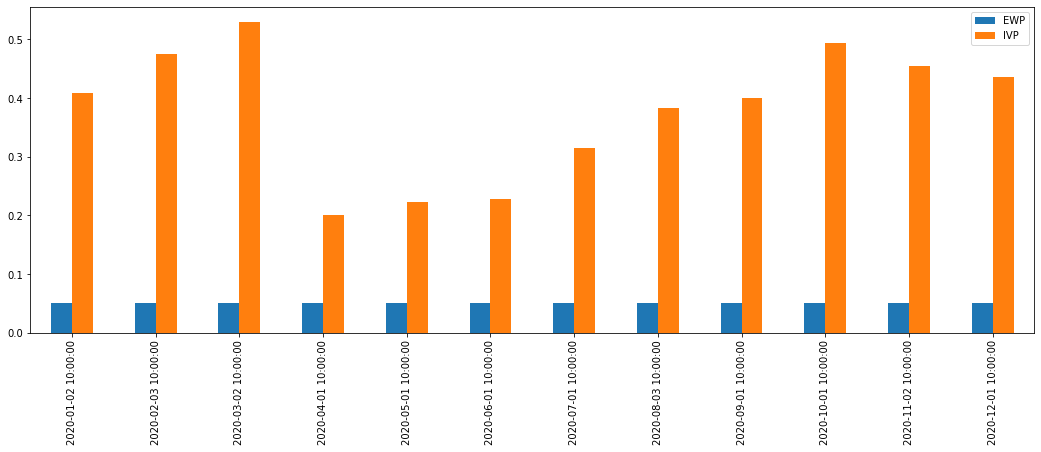
\includegraphics[width=1.15\textwidth]{bilder/nHHI_EWP_and_IVP.png}
            \caption{nHHI over Time}
            \label{fig:nHHI_EWP_and_IVP}
        \end{figure}
        
        Table \ref{tab:ewp_ivp_sharpe_turnover} presents the risk-adjusted returns and turnover of both naive strategies. Inverse variance portfolios achieve a Sharpe ratio almost three times higher than the Sharpe ratio of the equal weight portfolio. The turnover of the IVP is also higher than the turnover of the EWP by a factor of 2.
        
        % Data
        \begin{table}[h!]
            \centering
            \begin{tabular}{crr}
             \textbf{Portfolio Optimisation Method} & \textbf{Sharpe Ratio} & \textbf{Turnover} \\
             \hline
             EWP & 0.438 & 0.003634 \\
             IVP & 1.221 & 0.007396
            \end{tabular}
            \caption{Sharpe Ratio and Turnover Figures}
            \label{tab:ewp_ivp_sharpe_turnover}
        \end{table}
        